\documentclass{article}
\usepackage[utf8]{inputenc}
\usepackage[spanish]{babel}
\usepackage{lipsum}
\usepackage{graphicx}
\usepackage{xcolor}
\usepackage{hyperref}
\usepackage{amsfonts}
\usepackage{amssymb}
\usepackage{amsmath}


\title{Pruebas con Git}
\author{Nicolas Cardona Ramirez}
\date{\today}

\begin{document}
	
	\maketitle
	
	\section{Video 2: Primeros pasos en Git}
	
	
	Para iniciar el Git se utiliza lo siguiente:
	\begin{enumerate}
		\item \textcolor{red}{git config --global user.name} seguido del usuario entre comillas
		\item \textcolor{red}{git config --global user.email} seguido del email entre comillas
		\item \textcolor{red}{git config --global color.ui true} para habilitar los colores dentro del código
	\end{enumerate}
	
	\section{Video 3: Iniciar el monitoreo}
	
	\begin{itemize}
		\item Con el comando \textcolor{blue}{git init}, para iniciar el rastreo del proyecto
		\item Con \textcolor{blue}{git status} se muestran las modificaciones del proyecto
		\item Para añadir los archivos a la sincronización se utiliza el comando \textcolor{blue}{git add}
		\item Para agregar todo al proyecto se utliza \textcolor{blue}{git add -A}
		\item Para agregar se utiliza el comando \textcolor{blue}{git commit -m} y un mensaje entre comillas para identificar la modificación
		\item Para ver una lista con los comentarios se utiliza el comando \textcolor{green}{git log}
		\item Ahora para viajar entre versiones, se crea un último commit, se utiliza el git log para copiar el código del commit y se utiliza el comando \textcolor{green}{git checkout} con el código del commit. Para ver el código en su totalidad se utiliza \textcolor{green}{git chechout master} para devolver a la versión deseada
		\item Para ``Matar los commit" se utiliza el comando \textcolor{green}{git reset} las el código del commit, el cuál se subdivide en \textcolor{blue}{git reset --soft}, el cúal no se mete con el código, esta el \textcolor{blue}{git reset --mixed} y está el comando \textcolor{blue}{git reset --hard} que borra absolutamente todo
		\item El comando \textcolor{green}{git log $>$ commits.txt} crea un documento de texto con cada uno de los commits
		\item El comando \textcolor{blue}{git help} da un pequño manual para el uso de git, si se quiere ser mas específico se utiliza git help + el nombre del comando
		
	\end{itemize}


	\section{Video 4: Ramas y Funciones}
	
	Head = Actual commit
	
	\begin{itemize}
	\item Para crear una rama se utiliza el comando \textcolor{blue}{git branch $+$ nombre de la rama}
	\item Para moverse entre ramas se utiliza el comando \textcolor{blue}{git checkout + el nombre de la rama}
	\item Para absorber una rama se utiliza el comando \textcolor{blue}{git merge} para absorber todos los commits de la rama de prueba
	\item Fast-Forward solo hace la fusion sin preguntar nada
	\item Manual Merge los cambios tienen que pasar por nosotros
	\item Para crear y cambia automaticamente a una nueva rama se utiliza el comando \textcolor{blue}{git checkout -b nueva rama}
	\end{itemize}

	\section{Video 5: GitHub}
	
	\begin{itemize}
		
	\item El comando \textcolor{green}{git clone} toma un proyecto de GitHub y lo pasa a la computadora
	\item El comando \textcolor{green}{git remote add origin} vincula el proyecto local con nuestro proyecto remoto
	\item Para comprobar el vinculo se utiliza el comando \textcolor{green}{git remote -v}
	\item Para desvincular se utiliza \textcolor{green}{git remote remove origin}
	\item Para sincronizar se utiliza \textcolor{green}{git push origin + la rama a pasar}
	\item Para hacer una prueba con las ramas en GitHub
	\end{itemize}
	
	\subsection{Issues, Milestones y Labels}
	
	\begin{itemize}
		\item Los \textcolor{red}{Issues} se utilizan para arreglar errores o algo que nos hace falta
		\item Los \textcolor{red}{Milestones} son grupos de Issues que se aplican para un proyecto, característica o periodo de tiempo
		\item Los \textcolor{red}{Labels} son etiquetas para los Issues
	\end{itemize}

	
	\section{Video 6: Tags}
	
	\begin{itemize}
		\item Los \textcolor{blue}{Tags} son etiquetas para identificar la versión del archivo o historia en nuestro proyecto
		\item Para modificar el nombre de un commit se utiliza el comando \textcolor{red}{git commit $-amend -m ``nuevo/ nombre"$}
		\item El comando \textcolor{red}{git push origin master -f} obliga a GitHub a tomar las modificaciones en los commit
		\subsection{Tags}
		\item Las \textcolor{blue}{Tags anotadas} son almacenadas como objetos completos dentro de la base de Git y contienen más información con el comando \textcolor{blue}{git tag -a -m$``"$}
		\item Las \textcolor{red}{Tags Ligeras} contienen menos información
		\item Para agregar Tags a commits dentro del proyecto se utiliza el comando \textcolor{blue}{git tag -a v0.7 -m "Version 0.7" $+$ el código SHA}
		\item Para compartir las tags en GitHub se utiliza el comando \textcolor{blue}{git push origin $+$ el nombre del tag}
		\item Para agregar todos los tags de golpe se utiliza el comando \textcolor{blue}{git push origin --tags}
	\end{itemize}

	\section{Video 7: WorkFlows}
	
		\begin{itemize}
		\item Crear organizaciones para el trabajo en equipo
		\item Para agregar una persona, se busca su nick o su correo y se le otorgar permisos de edición
		\item La otra persona clona el proyecto de la misma manera
		\item Para ver las ramas ocultar y observar la rama origin/master se utiliza el comando \textcolor{green}{git branch -a}
		\item Para pasar los commit de Omar y de Filli se utiliza el comando \textcolor{green}{git fetch} (Ver Fig. \ref{fetch}). El flujo es el siguiente: Con el comando \textcolor{red}{fetch origin} se sube todo al origin/master y con el comando  \textcolor{red}{merge origin/master} se absorben esos cambio; una vez se tienen los cambios, se sube de nuevo al origin master con el comando push
		\item Se debe recordar que se debe cambiar el tipo de conexión remota, del usuario del repositorio del chest al repositorio de la organización con el comando \textcolor{green}{git remote remove -v} y se verifica con el comando \textcolor{green}{git remote -v} y se pone de nuevo \textcolor{green}{git remote add origin $+$ código de la organización}
		
	\end{itemize}

	\begin{figure}[t!]
		\centering
		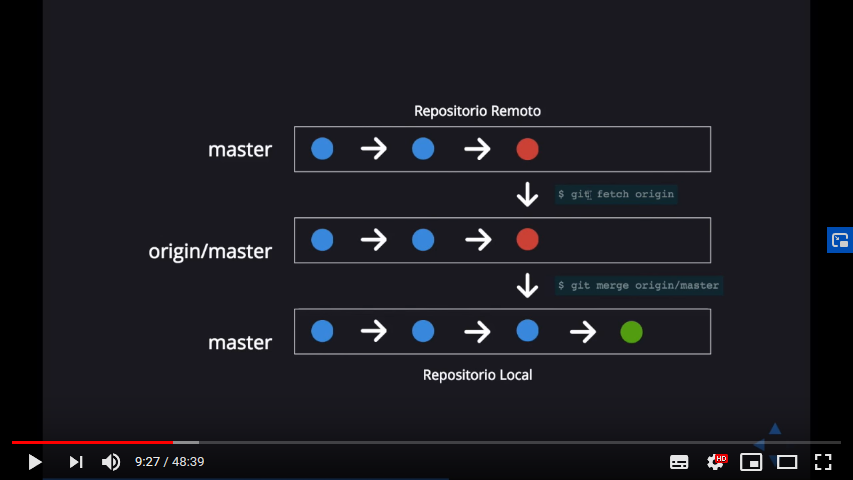
\includegraphics[width = 100mm]{imagenes/fetch2}
		\caption{Comando Fetch}
		\label{fetch}
	\end{figure}

		\begin{figure}[th]
		\centering
		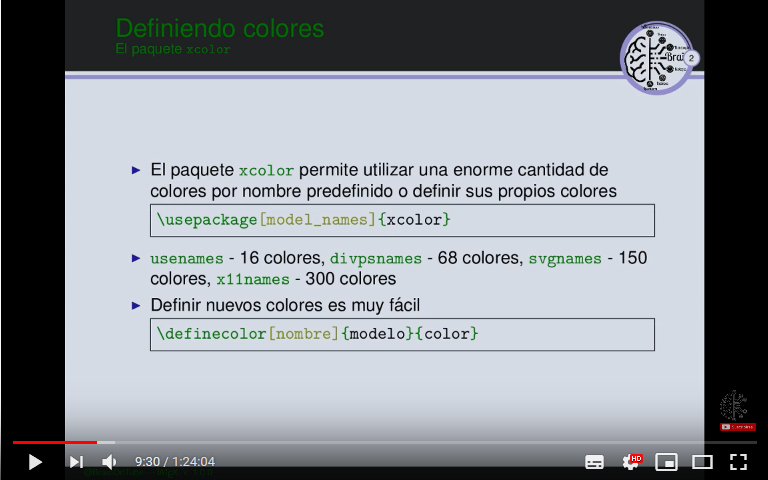
\includegraphics[width = 100mm]{imagenes/Colores}
		\caption{Colores \LaTeX{}}
		\label{colores}
	\end{figure}

\end{document}
